\documentclass[main]{subfiles}





\begin{document}
\subsection{Идея}

Как было сказано в анализе проблемы, именно база данных слов русского языка, разработанная В.А. Дзюбенко, стала базовым инструментом для решения задачи при помощи предложенного нами подхода.

Мы дополнили существующую базу данных несколькими таблицами; её схема представлена на рис. \ref{img1}, а структура таблиц расписана в приложении\ref{app:A}.


\begin{figure}[h]
	\begin{minipage}[h]{\linewidth}
			\captionsetup{format=hang,labelsep = endash}
		\center{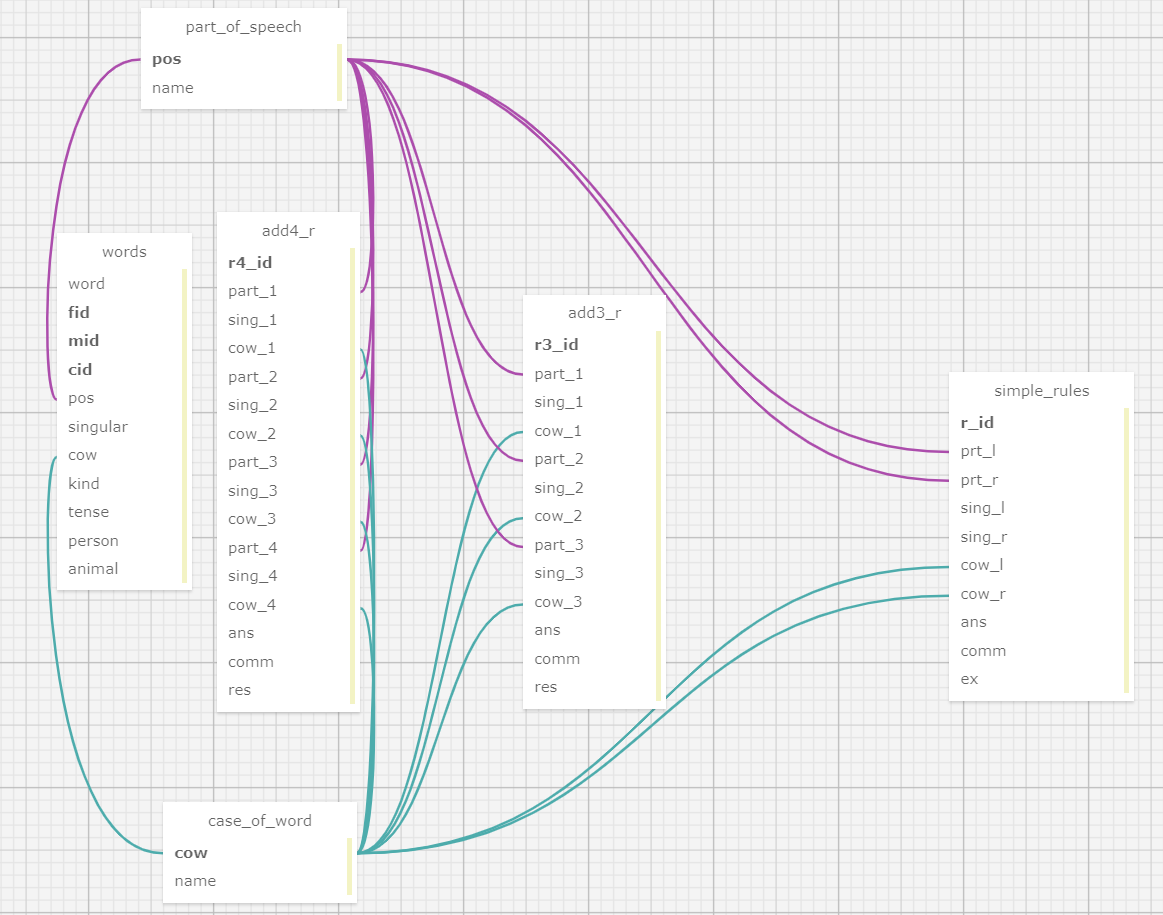
\includegraphics[width=\linewidth]{im1}}
		\caption{Концептуальная схема усовершенствованной базы данных}\label{img1}
	\end{minipage}
\end{figure}

В рамках предложенного нами подхода мы описываем слово при помощи трёх параметров: часть речи, число и падеж. Нами было выявлено около сотни правил для словосочетаний длины $2$, $3$ или $4$, по которым можно определить, нет ли ошибки в согласовании единственного и множественного числа? Полученные результаты представлены в приложении \ref{app:B}

В основе предложенного нами подхода лежит гипотеза, согласно которой одно и то же предложение являться и не являться ошибочным одновременно с точки зрения согласования единственного и множественного числа не может. 

Также считаем, что в предложении нет орфографических, пунктуационных и др. ошибок, поскольку данная задача была успешно решена, например, компанией LanguageTooler GmbH \cite{langt}.

\subsection{Подготовительный этап}
На вход программе подаётся предложение, состоящее из существительных, местоимений, личных глаголов или (и) инфинитивов (с, возможно, перечислением инфинитивов или личных глаголов с зависимыми словами, принадлежащим указанным частям речи). 

Полученное предложение передаётся функции space(), которая преобразует считанную строку в список. Механизм её работы описывает алгоритм \ref{alg1}.

\begin{algorithm}
	\caption{-- Предварительная обработка входных данных}\label{alg1}
	\begin{algorithmic}[1]
		\Function{space}{str1}
		\State str1 $\gets$ str1.lower() \Comment{Приводим полученную строку к нижнему регистру}
		\State str2 $\gets $ <<>> \Comment{В этой переменной будет храниться преобразованная строка}
		\State l $\gets$ len(str1)
		\For{\textbf{from} $i=0$ \textbf{to} $l - 1$} 
		\If{str1$[i] \in \{$<<.>>; <<,>> $\}$  }
		\State str2 $\gets$ str2 $+$ << >>
		\EndIf
		\State str2 $\gets$ str2 $+$ str1$[i]$
		\EndFor
		\If{str2[len(str2) $- 1$] $=$ << >>}
		\State str2 $\gets$ str2[ : len(str2) $- 1$] \Comment{Отбрасываем этот пробел}
		\EndIf
		\State\Return str2.split() \Comment{Возвращаем список, полученный из строки str2 разбиением её по пробелам}
		\EndFunction
	\end{algorithmic}
\end{algorithm}

Таким образом, функция space() возвращает список, состоящий из слов и знаков препинания исходной строки.

\subsection{Обработка предложения}

Итак, как было сказано выше, проверка согласования единственного и множественного числа в русском языке~--- процесс сложный: нужно учесть много критериев. 

Нами было принято решение декомпозировать задачу. 

Для начала (при наличии перечислений инфинитивов или личных личных глаголов) предложение упрощается: перечисление мы заменяем на инфинитив или личный глагол соответственно (параллельно проверяя, что внутри заменяемой части нет ошибок в согласовании единственного и множественного числа). Если же перечисления не обнаружено, сразу переходим к следующему этапу.

Затем проверяем предложение без перечислений при помощи разработанной нами системы правил. 

Согласно теореме Гёделя о неполноте, формальная арифметика либо противоречива, либо неполна \cite{forms}. Чтобы избежать противоречивости разработанной системы, мы включили лишь те правила, которые встречаются на практике, а не перебрали все возможные комбинации используемых нами параметров.

\subsubsection{Упрощение предложения}
Под упрощением мы будем понимать замену перечисления инфинитивов или личных глаголов одиночным инфинитивом или личным глаголом. 

За упрощение предложения отвечает функция comma(), которая принимает на вход список, полученный из исходного предложения при помощи функции space(), описанной выше; а возвращает список, в виде которого представлено упрощённое предложение. Функция comma() вызывается только в том случае, если в предложении есть <<и>> или <<или>>. Механизм её работы описывает алгоритм \ref{alg2}.

\begin{algorithm}
	\caption{-- Обработка перечислений}\label{alg2}
	\begin{algorithmic}[1]
		\Function{comma}{l} \Comment{l~--- подготовленная строка в виде списка}
		\State part $\gets [$ $]$ \Comment{Список значений параметра <<часть речи>> для данного слова (изначально пустой)}
		\State end$\gets (-1)$ \Comment{Индикатор нахождения начала перечисления}
		\State left $\gets (-1)$ \Comment{Левая и правая границы заменяемого участка изначально}
		\State right $\gets (-1)$\Comment{инициализируем невозможными значениями: $(-1)$}
		\State llen $\gets $len(l) \Comment{Длина исходного списка}
		\If{<<и>> $\in$ l}
		\State w$\gets$ <<и>>\Comment{w хранит союз, использующийся в перечислении}
		\ElsIf{<<или>> $\in$ l}
		\State w$\gets$ <<или>>
		\EndIf
		\State id1 $\gets$ l.index(w)\Comment{Записываем индекс w в списке} 
		\algstore{bkbreak}
	\end{algorithmic}
\end{algorithm}
В рамках установленных нами ограничений <<и>> или <<или>> могут быть использованы только для перечислений личных глаголов или инфинитивов.

\begin{algorithm}
	\caption{-- Продолжение алгоритма \ref{alg2}}\label{alg3}
	\begin{algorithmic}[1]
		\algrestore{bkbreak}
				\If{llen $>$ id1 $+ 1$}
		\State resp1 $\gets$ l[id1 $+ 1$].[pos, singular, cow] 
			\EndIf
		\If{llen $>$ id1 $+ 2$}
		\State resp2 $\gets$ l[id1 $+ 2$].[pos, singular, cow]
		\EndIf	
		\If{llen $>$ id1 $+ 3$}
		\State resp3 $\gets$ l[id1 $+ 3$].[pos, singular, cow] 
		\EndIf
		\If{llen $>$ id1 $+ 4$}
		\State resp4 $\gets$ l[id1 $+ 4$].[pos, singular, cow]
		\EndIf
		\If{id1 $-1 \ge 0$}
		\State resl1 $\gets$ l[id1 $-1$].[pos, singular, cow]
		\EndIf
		\If{id1 $-2 \ge 0$}
		\State resl2 $\gets$ l[id1 $-2$].[pos, singular, cow]
		\EndIf
		\If{id1 $-3 \ge 0$}
		\State resl3 $\gets$ l[id1 $-3$].[pos, singular, cow]
		\EndIf
		\If{id1 $-4 \ge 0$}
		\State resl1 $\gets$ l[id1 $-4$].[pos, singular, cow]
		\EndIf
		\If{id1 $-5 \ge 0$}
		\State resl5 $\gets$ l[id1 $-5$].[pos, singular, cow]
		\EndIf
		\If{id1 $-6 \ge 0$}
		\State resl6 $\gets$ l[id1 $-6$].[pos, singular, cow]
		\EndIf
		\If{id1 $-7\ge 0$}
		\State resl7 $\gets$ l[id1 $-7$].[pos, singular, cow]
		\EndIf
		\If{id1 $+1 <$ llen}
		\For{\textbf{from} $i=0$ \textbf{to} len(resp1)$- 1$}
		\If{resp1$[i][0]=$<<6>>} \Comment{Слово оказалось инфинитивом}
		\State part$\gets$ <<6>> \textbf{and} right $\gets$ id1 $+1$
				\EndIf
					\EndFor
					\If{right$=(-1)$}\Comment{Если же это не инфинитив}
					\For{\textbf{from} $i=0$ \textbf{to} len(resp1)$-1$}
					\If{resp1$[i][0]=$<<5>>}\Comment{Слово оказалось личным глаголом}
					\State right $\gets$id1$ + 1$ \textbf{and}  part $\gets$ <<5>>
					\State sng $\gets $l$[i][1]$ \Comment{Для личных глаголов важно число}
					\State \textbf{break}
							\EndIf
							\EndFor
									\EndIf
											\EndIf
		\algstore{bkbreak}
	\end{algorithmic}
\end{algorithm}

Таким образом, в результате исполнения блока \ref{alg3} будет определено, слова (словосочетания) какой части речи перечисляются (если в предложении присутствует перечисление с союзом <<и>>).

Заметим, что в случае перечисления с союзом <<и>> за союзом идёт слово той же части речи, что и остальные перечисляемые слова. Например: \textit{<<Он хотел \textbf{читать} книги, \textbf{рисовать} картины и \textbf{познавать} тайны мироздания>>}. Легко видеть, что в предложении перечисляются инфинитивы, и в то же время после союза <<и>> идёт инфинитив <<познавать>>.

Если перечисляются инфинитивы, то упрощение предложения идёт согласно алгоритму \ref{alg4}.

Прежде всего, нужно определить начало левого операнда <<и>>. В зависимости от длины буквосочетания, возможны различные варианты:
\begin{enumerate}
	\item Словосочетание длины $6$. Например, инф. + сущ. + сущ. + сущ. + сущ. + сущ.: \textit{<<Организовать проверку знаний требований охраны труда>>}.
	\item Словосочетание длины $5$. Например, инф. + сущ. + сущ. + сущ. + сущ.: \textit{<<Организовать проверку знаний основ программирования>>}.
	\item Словосочетание длины $4$. Например, инф. + инф. + сущ. + сущ.: \textit{<<Пойти спать сном младенца>>}.
	\item Словосочетание длины $3$. Например, инф. + сущ. + сущ.: \textit{<<Оценить игру слов>>}.
	\item Словосочетание длины $2$. Например, инф. + инф.: \textit{<<Пойти позавтракать>>}.
	\item Одиночный инфинитив. Например: \textit{<<Быть>>}.
\end{enumerate}
Итак, первым делом инициализируем левую границу заменяемого <<куска>> списка.
\begin{algorithm}
	\caption{-- Продолжение алгоритма \ref{alg3}}\label{alg4}
	\begin{algorithmic}[1]
		\algrestore{bkbreak}
		\If{part $=$<<6>>}\Comment{Если перечисляемая часть речи~--- инфинитив}
		\If{id1$-6\ge 0$ \textbf{and} left$=(-1)$ \textbf{and} <<,>>$\notin$ l$[$id1$ - 6:\,$ id1$]$} \Comment{Проверяем буквосочетания длины $6$}
		\For{\textbf{from} $i = 0$ \textbf{to} len(resl6)$-1$}
		\If{resl6$[i][0]=$part}
		\State r$\gets$ check(l$[$id1$-6$ : id1$]$)
		\If{<<N>>$\in $ r}
		\State \Return $[$<<он>>, <<писали>> $]$ \Comment{Заведомо неверное предложение}
		\ElsIf{<<Y>>$\in $ r}
		\algstore{bkbreak}
	\end{algorithmic}
\end{algorithm}

\begin{algorithm}
	\caption{-- Продолжение алгоритма \ref{alg4}}\label{alg5}
	\begin{algorithmic}[1]
		\algrestore{bkbreak}
		\State left $\gets$ id1$-6$ \Comment{Инициализировали границу левого операнда <<и>>}
		\State \textbf{break}
		\EndIf
		\EndIf
		\EndFor
		\EndIf
		\If{id1$-5\ge 0$ \textbf{and} left$=-1$ \textbf{and} <<,>>$\notin$ l$[$id1$ - 5:\,$ id1$]$}
		\For{\textbf{from} $i = 0$ \textbf{to} len(resl5)$-1$}
		\If{resl5$[i][0]=$part}
		\State r$\gets$ check(l$[$id1$-5$ : id1$]$)
		\If{<<N>>$\in $ r}
		\State \Return $[$<<он>>, <<писали>> $]$
		\ElsIf{<<Y>>$\in $ r}
		\State left $\gets$ id1$-5$ 
		\State \textbf{break}
		\EndIf
		\EndIf
		\EndFor
		\EndIf
		\If{id1$-4\ge 0$ \textbf{and} left$=-1$ \textbf{and} <<,>>$\notin$ l$[$id1$ - 4:\,$ id1$]$}
		\For{\textbf{from} $i = 0$ \textbf{to} len(resl4)$-1$}
		\If{resl4$[i][0]=$part}
		\State r$\gets$ check(l$[$id1$-4$ : id1$]$)
		\If{<<N>>$\in $ r}
		\State \Return $[$<<он>>, <<писали>> $]$
		\ElsIf{<<Y>>$\in $ r}
		\State left $\gets$ id1$-4$ 
		\State \textbf{break}
		\EndIf
		\EndIf
		\EndFor
		\EndIf
		\If{id1$-3\ge 0$ \textbf{and} left$=-1$ \textbf{and} <<,>>$\notin$ l$[$id1$ - 3:\,$ id1$]$}
		\For{\textbf{from} $i = 0$ \textbf{to} len(resl3)$-1$}
		\If{resl3$[i][0]=$part}
		\State r$\gets$ check(l$[$id1$-3$ : id1$]$)
	\If{<<N>>$\in $ r}
\State \Return $[$<<он>>, <<писали>> $]$
\ElsIf{<<Y>>$\in $ r}
\State left $\gets$ id1$-3$ 
\State \textbf{break}
\EndIf
\EndIf
\EndFor
		\EndIf
		\algstore{bkbreak}
	\end{algorithmic}
\end{algorithm}
Таким образом, в результате выполнения данного фрагмента кода будет определены границы левого и правого операндов союза.
\begin{algorithm}
	\caption{-- Продолжение алгоритма \ref{alg5}}\label{alg6}
	\begin{algorithmic}[1]
		\algrestore{bkbreak}	
		\If{id1$-2\ge 0$ \textbf{and} left$=-1$ \textbf{and} <<,>>$\notin$ l$[$id1$ - 2:\,$ id1$]$}
		\For{\textbf{from} $i = 0$ \textbf{to} len(resl2)$-1$}
		\If{resl2$[i][0]=$part}
		\State r$\gets$ check(l$[$id1$-2$ : id1$]$)
		\If{<<N>>$\in $ r}
		\State \Return $[$<<он>>, <<писали>> $]$
		\ElsIf{<<Y>>$\in $ r}
		\State left $\gets$ id1$-2$ 
		\State \textbf{break}
		\EndIf
		\EndIf
		\EndFor
		\EndIf
		\If{id1$-1\ge 0$ \textbf{and} left$=(-1)$}
		\For{\textbf{from} $i = 0$ \textbf{to} len(resl1)$-1$}
		\If{l$[i][0]=$part}
		\State left $\gets$ id1$-1$
		\State \textbf{break}
		\EndIf
		\EndFor
		\EndIf
		\EndIf
		\State Алгоритм \ref{alg7}
		\State Алгоритм \ref{alg11}
		\State Алгоритм \ref{alg12}
		\EndFunction
	\end{algorithmic}
\end{algorithm}

В алгоритмах \ref{alg5} и \ref{alg6} неоднократно фигурирует функция check(). В данном случае она используется для проверки предложения, не содержащего знаки пунктуации. Её описание будет в следующем параграфе.

Далее возможен один из двух вариантов:
\begin{itemize}
	\item Союз связывает только два слова или словосочетания, или слово и словосочетание.
	\item Союз используется для перечисления $3$ и более словосочетаний и (или) слов.
\end{itemize}

В первом случае предложение готово к упрощению: <<кусок>> от left до right заменяем единичным инфинитивом.

Во втором же случае необходимо продолжить анализ предложения, сдвигая левую границу заменяемого участка.

Для начала будем искать участки между двумя запятыми (при их наличии). Особенность данного этапа заключается в том, что между запятыми может оказаться ошибочное словосочетание,~--- потому фрагменты между запятыми нужно также проверять на согласованность.

Также важен порядок рассмотрения случаев: в первую очередь следует искать самые <<короткие>> словосочетания между запятыми (иначе можем <<захватить>> подстроку с запятыми). Этот и последующие этапы описаны в алгоритме \ref{alg7}.

\begin{algorithm}
	\caption{-- Фрагмент алгоритма \ref{alg6}}\label{alg7}
	\begin{algorithmic}[1]
	\While{<<,>>$\in$ l$[1:$ left $]$}\Comment{Пока есть запятые}
	\If{l$[$left $-1]=$ <<,>> \textbf{and} l$[$left $-3]=$ <<,>>} \Comment{Между запятыми одно слово}
	\State res1$\gets$ l$[$left$-2]$.[pos, singular, cow]
	\For{\textbf{from} $i = 0$ \textbf{to} len(res1)}
	\If{res1$[i][0]=$part}
	\State left$\gets$ left$-2$
	\State \textbf{break}
	\EndIf
	\EndFor
	\ElsIf{l$[$left $-1]=$ <<,>> \textbf{and} l$[$left $-4]=$ <<,>>} \Comment{Между запятыми словосочетание из двух слов}
	\State  res1$\gets$ l$[$left$-3]$.[pos, singular, cow]
	\For{\textbf{from} $i = 0$ \textbf{to} len(res1)}
	\If{res1$[i][0]=$part}
	\State r $\gets$ check(l$[$left$-3:$ left$-1 ]$)
	\If{<<N>> $\in$ r}
	\State \Return $[$<<он>>, <<писали>> $]$
	\ElsIf{<<Y>> $\in$ r}
	\State left$\gets$ left$-3$
	\State \textbf{break}
	\EndIf
	\EndIf
	\EndFor
	\ElsIf{l$[$left $-1]=$ <<,>> \textbf{and} l$[$left $-5]=$ <<,>>}
	\State  res1$\gets$ l$[$left$-4]$.[pos, singular, cow]
	\For{\textbf{from} $i = 0$ \textbf{to} len(res1)}
	\If{res1$[i][0]=$part}
	\State r $\gets$ check(l$[$left$-4:$ left$-1 ]$)
	\If{<<N>> $\in$ r}
	\State \Return $[$<<он>>, <<писали>> $]$
	\ElsIf{<<Y>> $\in$ r}
	\State left$\gets$ left$-4$
	\State \textbf{break}
	\EndIf
	\EndIf
	\algstore{bkbreak}
	\end{algorithmic}
	\end{algorithm}

\begin{algorithm}
	\caption{-- Продолжение алгоритма \ref{alg7}}\label{alg8}
	\begin{algorithmic}[1]
		\algrestore{bkbreak}
			\EndFor
			\ElsIf{l$[$left $-1]=$ <<,>> \textbf{and} l$[$left $-6]=$ <<,>>}
		\State  res1$\gets$ l$[$left$-5]$.[pos, singular, cow]
		\For{\textbf{from} $i = 0$ \textbf{to} len(res1)}
			\If{res1$[i][0]=$part}
			\State r $\gets$ check(l$[$left$-5:$ left$-1 ]$)
			\If{<<N>> $\in$ r}
			\State \Return $[$<<он>>, <<писали>> $]$
		\ElsIf{<<Y>> $\in$ r}
			\State left$\gets$ left$-5$
		\State \textbf{break}
		\EndIf
			\EndIf
		\EndFor
		\ElsIf{l$[$left $-1]=$ <<,>> \textbf{and} l$[$left $-7]=$ <<,>>}
		\State  res1$\gets$ l$[$left$-6]$.[pos, singular, cow]
		\For{\textbf{from} $i = 0$ \textbf{to} len(res1)}
		\If{res1$[i][0]=$part}
		\State r $\gets$ check(l$[$left$-6:$ left$-1 ]$)
		\If{<<N>> $\in$ r}
		\State \Return $[$<<он>>, <<писали>> $]$
		\ElsIf{<<Y>> $\in$ r}
		\State left$\gets$ left$-6$
		\State \textbf{break}
		\EndIf
		\EndIf
		\EndFor
		\ElsIf{l$[$left $-1]=$ <<,>> \textbf{and} l$[$left $-8]=$ <<,>>}
		\State  res1$\gets$ l$[$left$-7]$.[pos, singular, cow]
		\For{\textbf{from} $i = 0$ \textbf{to} len(res1)}
		\If{res1$[i][0]=$part}
		\State r $\gets$ check(l$[$left$-7:$ left$-1 ]$)
		\If{<<N>> $\in$ r}
		\State \Return $[$<<он>>, <<писали>> $]$
		\ElsIf{<<Y>> $\in$ r}
		\State left$\gets$ left$-7$
		\State \textbf{break}
		\EndIf
		\EndIf
		\EndFor
		\Else \State Алгоритм \ref{alg9}
		\EndIf
			\EndWhile
		%\algstore{bkbreak}
	\end{algorithmic}
\end{algorithm}
\newpage

Итак, в результате работы фрагментов \ref{alg7} и \ref{alg8} будет сдвинута граница до <<первой>> запятой.

Следующий этап~--- поиск начала перечисления. Соответствующий фрагмент описан алгоритмом \ref{alg9}.

Индикатор end отвечает за нахождение начала перечисления (изначально был инициализирован $(-1)$, а после нахождения начала перечисления будет равен $1$). Как и раньше, проверяем первый найденную подстроку на выполнение правил в ней.
\begin{algorithm}
	\caption{-- Фрагмент алгоритма \ref{alg8}}\label{alg9}
	\begin{algorithmic}[1]
	\If{left$-2\ge 0$\textbf{ and }l$[$left$-1]=$<<,>> \textbf{and} end$=(-1)$}
	\State res1$\gets$ l$[$left$-2]$.[pos, singular, cow]
	\For{\textbf{from} $i = 0$ \textbf{to} len(res1)$ - 1$}
	\If{res1$[i][0]=$<<6>>}
	\State left$\gets$ left$-2$
	\State \textbf{break}
	\EndIf
	\EndFor
	\EndIf
	\If{left$-3\ge 0$\textbf{ and }l$[$left$-1]=$<<,>> \textbf{and} end$=(-1)$}
	\State res1$\gets$ l$[$left$-3]$.[pos, singular, cow]
	\For{\textbf{from} $i = 0$ \textbf{to} len(res1)$ - 1$}
	\If{res1$[i][0]=$<<6>>}
	\State r $\gets$ check(l$[$left$-3:$ left$-1]$)
	\If{<<N>>$\in$ r}
	\State \Return $[$<<он>>, <<писали>> $]$
	\ElsIf{<<Y>> $\in$ r}
	\State left$\gets$ left$-3$
	\State end $\gets 1$
	\State \textbf{break}
	\EndIf
	\EndIf
	\EndFor
	\EndIf
	\If{left$-4\ge 0$\textbf{ and }l$[$left$-1]=$<<,>> \textbf{and} end$=(-1)$}
	\State res1$\gets$ l$[$left$-4]$.[pos, singular, cow]
	\For{\textbf{from} $i = 0$ \textbf{to} len(res1)$ - 1$}
	\If{res1$[i][0]=$<<6>>}
	\State r $\gets$ check(l$[$left$-4:$ left$-1]$)
	\If{<<N>>$\in$ r}
	\State \Return $[$<<он>>, <<писали>> $]$
	\ElsIf{<<Y>> $\in$ r}
	\State left$\gets$ left$-4$
	\State end $\gets 1$
	\State \textbf{break}
\EndIf
	\algstore{bkbreak}
	\end{algorithmic}
\end{algorithm}

\begin{algorithm}
	\caption{-- Продолжение алгоритма \ref{alg9}}\label{alg10}
	\begin{algorithmic}[1]
		\algrestore{bkbreak}
			\EndIf
			\EndFor
			\EndIf
				\If{left$-5\ge 0$\textbf{ and }l$[$left$-1]=$<<,>> \textbf{and} end$=(-1)$}
			\State res1$\gets$ l$[$left$-5]$.[pos, singular, cow]
			\For{\textbf{from} $i = 0$ \textbf{to} len(res1)$ - 1$}
			\If{res1$[i][0]=$<<6>>}
			\State r $\gets$ check(l$[$left$-5:$ left$-1]$)
			\If{<<N>>$\in$ r}
			\State \Return $[$<<он>>, <<писали>> $]$
			\ElsIf{<<Y>> $\in$ r}
			\State left$\gets$ left$-5$
			\State end $\gets 1$
			\State \textbf{break}
			\EndIf
			\EndIf
			\EndFor
			\EndIf
			\If{left$-6\ge 0$\textbf{ and }l$[$left$-1]=$<<,>> \textbf{and} end$=(-1)$}
			\State res1$\gets$ l$[$left$-6]$.[pos, singular, cow]
			\For{\textbf{from} $i = 0$ \textbf{to} len(res1)$ - 1$}
			\If{res1$[i][0]=$<<6>>}
			\State r $\gets$ check(l$[$left$-6:$ left$-1]$)
			\If{<<N>>$\in$ r}
			\State \Return $[$<<он>>, <<писали>> $]$
			\ElsIf{<<Y>> $\in$ r}
			\State left$\gets$ left$-6$
			\State end $\gets 1$
			\State \textbf{break}
			\EndIf
			\EndIf
			\EndFor
			\EndIf
			\If{left$-7\ge 0$\textbf{ and }l$[$left$-1]=$<<,>> \textbf{and} end$=(-1)$}
			\State res1$\gets$ l$[$left$-7]$.[pos, singular, cow]
			\For{\textbf{from} $i = 0$ \textbf{to} len(res1)$ - 1$}
			\If{res1$[i][0]=$<<6>>}
			\State r $\gets$ check(l$[$left$-7:$ left$-1]$)
			\If{<<N>>$\in$ r}
			\State \Return $[$<<он>>, <<писали>> $]$
			\ElsIf{<<Y>> $\in$ r}
			\State left$\gets$ left$-7$
			\State end $\gets 1$
			\State \textbf{break}
			\EndIf
			\EndIf
			\EndFor
			\EndIf
		%\algstore{bkbreak}
	\end{algorithmic}
\end{algorithm}

Итак, после выполнения алгоритма \ref{alg9} будут определены границы заменяемой подстроки, после чего необходимо вставить вместо перечисления инфинитивов одиночный инфинитив. Нами было выбрано слово \textit{<<учить>>} (для данной цели можно было выбрать любой инфинитив, так как мы решаем проблему согласования единственного и множественного числа).

\begin{algorithm}
	\caption{-- Фрагмент алгоритма \ref{alg6}}\label{alg11}
	\begin{algorithmic}[1]
		\State l$\gets$ l$[\,:$ left$] +$ $[$<<учить>>$]+$ l$[$ right$+1:\, $id1$]$
	\end{algorithmic}
\end{algorithm}

Если же при помощи союза <<и>> перечисляются личные глаголы, то упрощение идёт согласно алгоритму \ref{alg12}. В зависимости от длины буквосочетания, возможны различные варианты словосочетаний:
\begin{enumerate}
	\item Словосочетание длины $7$. Например, личн. глаг. + инф. + сущ. + сущ. + сущ.~+ +~сущ.: \textit{<<Хотел организовать проверку знаний требований охраны труда>>}.
	\item Словосочетание длины $6$. Например, личн. глаг. + сущ. + сущ. + сущ. + сущ.~+ +~сущ.: \textit{<<Организовывал проверку знаний требований охраны труда>>}.
	\item Словосочетание длины $5$. Например, личн. глаг. + инф. + сущ. + сущ. + сущ.: \textit{<<Хотел изучить основы теории кодирования>>}.
	\item Словосочетание длины $4$. Например, личн. глаг. + сущ. + сущ. + сущ.: \textit{<<Изучил основы теории кодирования>>}.
	\item Словосочетание длины $3$. Например, личн. глаг. + инф. + сущ.: \textit{<<Желает знать правду>>}.
	\item Словосочетание длины $2$. Например, личн. глаг. + инф.: \textit{<<Желает знать>>}.
	\item Одиночный личный глагол. Например: \textit{<<Желать>>}.
\end{enumerate}

Во многом алгоритм обработки перечислений личных глаголов похож на алгоритм обработки перечислений инфинитивов.

Однако, в отличие от последних, для личных глаголов определено понятие числа. И в данной ситуации возникает\textit{\textbf{ проблема омографии}}. Так, слово \textit{<<спАли>>}~--- личный глагол во множественном числе, а \textit{<<спалИ>>}~--- личный глагол в единственном числе. В самом деле, данные слова совпадают по написанию, но различны по звучанию и значению. Заметим, что в единственном числе слово интерпретируется тогда и только тогда, когда оно  в повелительном наклонении. Легко видеть, что на множестве рассматриваемых в данной работе частей речи перечисляются личные глаголы в повелительном наклонении тогда и только тогда, когда предложение начинается с глагола в повелительном наклонении. Потому сразу определим, является ли первое слово глаголом. Если да, однозначно ли определяется его число.
\begin{algorithm}
	\caption{-- Продолжение алгоритма \ref{alg6}}\label{alg12}
	\begin{algorithmic}[1]
		\If{part$=$<<5>>}
		\State sng0 $\gets [\,]$\Comment{Для определения числа первого слова в предложении}
		\State pov $\gets (-1)$\Comment{Индикатор повелительного наклонения}
		\State res0$\gets$ l$[0].[$cow, singular, cow$]$
		\State end$\gets (-1)$
		\For{\textbf{from} $i = 0$ \textbf{to} len(res0)$ - 1$}
		\If{res0$[i][0]=$<<5>>}
		\State sng0 $\gets$ sng0 + list(res0$[i][1]$)
		\EndIf
		\EndFor
		\State sng0 $\gets$ list(set(sng0))
		\If{len(sng0)$ > 1$}
		\State pov $\gets 1$
		\State sng $\gets $<<Y>> \Comment{Считаем единственным число перечисляемых личных глаголов} 
		\EndIf
		\If{id1$-7\ge 0$ \textbf{and} left$=(-1)$ \textbf{and} <<,>>$\notin$ l$[$id1$ - 7:\,$ id1$]$}
		\State sng1 $\gets [\, ]$ \Comment{Для записи возможных значений числа}
		\State r $\gets [\, ]$ \Comment{Для записи результата проверки по системе правил}
		\For{\textbf{from} $i=0$ \textbf{to} len(resl7)$ - 1$}
		\If{resl7$[i][0]=$part}
		\State sng1$\gets$ sng1 $+$ list(resl7$[i][1]$)
		\State r$\gets$ r $+$ list(check(l$[$id1$-7\, :\, $ id1 $]$))
		\EndIf
		\EndFor
		\If{len(sng1)$ > 0$} \Comment{Если словосочетание действительно начинается с личного глагола}
		\If{(len(sng1)$=1$ \textbf{and} sng $\in$ sng1 \textbf{and} <<Y>>$\in$ r) \textbf{or} (len(sng1)$>1$ \textbf{and} (sng$=$<<N>> \textbf{or} pov$=1$) \textbf{and} <<Y>> $\in$ r)}
		\State left$\gets$ id1$-7$
		\Else
		\State \Return $[$<<он>>, <<писали>> $]$
		\EndIf
		\EndIf
		\EndIf
		\algstore{bkbreak}
	\end{algorithmic}
\end{algorithm}

Здесь следует рассмотреть решение проблемы омографии. В строках 6~--~32 алгоритма \ref{alg12}. Для начала проверяем, является ли первое слово рассматриваемого предложения личным глаголом, число которого определено неоднозначно. Это имеет значение, поскольку в рамках поставленных ограничений если в предложении есть личные глаголы в повелительном наклонении, то с одного из них оно начинается. Например: \textit{<<Учите математику, высыпайтесь и будьте людьми>>}.

Далее проверяем, что рассматриваемое словосочетание нужной длины и не содержит запятых. Если вдруг первое слово данного словосочетания оказалось личным глаголом, то мы запоминаем какого оно числа может быть; а также проверяем данное словосочетание на наличие или отсутствие ошибок в согласовании единственного и множественного числа.

Словосочетание не содержит ошибок в следующих случаях:\begin{enumerate}
	\item Число личного глагола опрелеляется однозначно и совпадает с числом правого операнда союза, проверка словосочетания на наличие ошибок в согласовании единственного и множественного числа прошла успешно (ошибок и незнакомых сочетаний не обнаружено).
	\item Число личного глагола определяется неоднозначно, и имеет место повелительное наклонение.
	\item Число личного глагола определяется неоднозначно, первое слово в предложении не является личным глаголом в повелительном наклонении и перечисляются личные глаголы во множественном числе.
\end{enumerate}

Это мы и проверяем. В остальных случаях возвращаем заведомо неверное предложение. Совершенно аналогично рассматриваются словосочетания меньшей длины:

\begin{algorithm}
	\caption{-- Продолжение алгоритма \ref{alg12}}\label{alg13}
	\begin{algorithmic}[1]
		\algrestore{bkbreak}
		\If{id1$-6\ge 0$ \textbf{and} left$=(-1)$ \textbf{and} <<,>>$\notin$ l$[$id1$ - 6:\,$ id1$]$}
		\State sng1 $\gets [\, ]$ 
		\State r $\gets [\, ]$ 
		\For{\textbf{from} $i=0$ \textbf{to} len(resl6)$ - 1$}
		\If{resl6$[i][0]=$part}
		\State sng1$\gets$ sng1 $+$ list(resl6$[i][1]$)
		\State r$\gets$ r $+$ list(check(l$[$id1$-6\, :\, $ id1 $]$))
		\EndIf
		\EndFor
		\If{len(sng1)$ > 0$} 
		\algstore{bkbreak}
	\end{algorithmic}
\end{algorithm}
\newpage
\begin{algorithm}
	\caption{-- Продолжение алгоритма \ref{alg13}}\label{alg14}
	\begin{algorithmic}[1]
		\algrestore{bkbreak}
		\If{(len(sng1)$=1$ \textbf{and} sng $\in$ sng1 \textbf{and} <<Y>>$\in$ r) \textbf{or} (len(sng1)$>1$ \textbf{and} (sng$=$<<N>> \textbf{or} pov$=1$) \textbf{and} <<Y>> $\in$ r)}я
		\State left$\gets$ id1$-6$
		\Else
		\State \Return $[$<<он>>, <<писали>> $]$
		\EndIf
		\EndIf
		\EndIf
		\If{id1$-5\ge 0$ \textbf{and} left$=(-1)$ \textbf{and} <<,>>$\notin$ l$[$id1$ - 5:\,$ id1$]$}
		\State sng1 $\gets [\, ]$ 
		\State r $\gets [\, ]$
		\For{\textbf{from} $i=0$ \textbf{to} len(resl5)$ - 1$}
		\If{resl5$[i][0]=$part}
		\State sng1$\gets$ sng1 $+$ list(resl5$[i][1]$)
		\State r$\gets$ r $+$ list(check(l$[$id1$-5\, :\, $ id1 $]$))
		\EndIf
		\EndFor
		\If{len(sng1)$ > 0$}
		\If{(len(sng1)$=1$ \textbf{and} sng $\in$ sng1 \textbf{and} <<Y>>$\in$ r) \textbf{or} (len(sng1)$>1$ \textbf{and} (sng$=$<<N>> \textbf{or} pov$=1$) \textbf{and} <<Y>> $\in$ r)}
		\State left$\gets$ id1$-5$
		\Else
		\State \Return $[$<<он>>, <<писали>> $]$
		\EndIf
		\EndIf
		\EndIf
		\EndIf
		%\algstore{bkbreak}
	\end{algorithmic}
\end{algorithm}


\subsubsection{Непосредственная проверка предложения}
\subsection{Примеры работы алгоритма}
\end{document}